\documentclass[11pt]{article}

\usepackage[utf8]{inputenc}
\usepackage[T1]{fontenc}
\usepackage{amsmath,amssymb,amsthm}
\usepackage{graphicx}
\usepackage{hyperref}
\usepackage{xcolor}
\usepackage{tikz}
\usetikzlibrary{decorations.pathreplacing}
\usepackage{enumitem}
\usepackage{booktabs}
\usepackage{geometry}
\geometry{margin=1in}

% Theorem environments
\newtheorem{theorem}{Theorem}
\newtheorem{lemma}[theorem]{Lemma}
\newtheorem{corollary}[theorem]{Corollary}
\newtheorem{definition}[theorem]{Definition}
\newtheorem{remark}[theorem]{Remark}

% Custom commands
\newcommand{\N}{\mathbb{N}}
\newcommand{\R}{\mathbb{R}}
\newcommand{\K}{\mathrm{K}}

\title{\textbf{Ph'nglui mglw'nafh Cthulhu R'lyeh wgah'nagl fhtagn:} \\[0.5em]
\large A Rigorous Proof of Lovecraftian Horror \\
from Kolmogorov Complexity}

\author{
  Sijie Wang\thanks{The author's sanity was partially lost during the preparation of this manuscript.} \\
  % \textit{Miskatonic University} \\
  % \texttt{ia-ia@cthulhu.fhtagn}
}

\date{SIGBOVIK 2026}

\begin{document}

\maketitle

\begin{abstract}
We prove that H.P. Lovecraft was mathematically correct.
Using Hutter's definition of intelligence as compression and the well-foundedness of the natural numbers,
we demonstrate that there necessarily exist intelligences that cannot be understood by any intelligence.
We call such entities \emph{Cthulhu objects}.
Furthermore, we show that \emph{most} objects in the universe are Cthulhu objects,
establishing cosmic horror as the default state of reality.
Our results unify Lovecraftian literature with G\"odel's incompleteness, Turing's undecidability,
and Lawvere's fixed point theorem under a single framework of diagonal despair.
\end{abstract}

\section{Introduction}

\begin{quote}
\textit{``The most merciful thing in the world, I think, is the inability of the human mind to correlate all its contents.''}
--- H.P. Lovecraft, \textit{The Call of Cthulhu} (1926)
\end{quote}

Lovecraft's work is often dismissed as mere fiction. In this paper, we prove he was doing mathematics.

Following Hutter's seminal work on universal intelligence \cite{hutter2007universal},
we adopt the definition that \textbf{intelligence is compression}:
to understand something is to find a shorter description of it.

We then ask: can everything be understood?

The answer, unfortunately for our sanity, is \textbf{no}.

\section{Preliminaries}

\begin{definition}[Kolmogorov Complexity]
For a string $x$, the Kolmogorov complexity $\K(x)$ is:
\[
\K(x) = \min \{ |p| : U(p) = x \}
\]
where $U$ is a universal Turing machine and $|p|$ is the length of program $p$.
\end{definition}

\begin{definition}[Intelligence, after Hutter \cite{hutter2007universal}]
Intelligence is the ability to compress: to understand $X$ is to find a description of $X$ shorter than $X$ itself.
\end{definition}

\begin{definition}[Incompressible]
An object $L$ is \emph{incompressible} if $\K(L) = |L|$, i.e., no description is shorter than $L$ itself.
\end{definition}

\section{The Compression Chain}

\begin{lemma}[Descending Chain]
For any object $X$, the compression operation produces a description no longer than $X$:
\[
|\mathrm{compress}(X)| = \K(X) \leq |X|
\]
with equality if and only if $X$ is incompressible.
\end{lemma}

\begin{proof}
By definition of Kolmogorov complexity: $\K(X) \leq |X| + c$ for some constant $c$
(since $X$ itself is a description of $X$). For simplicity we absorb constants. \qed
\end{proof}

Consider the sequence:
\[
X \to \mathrm{compress}(X) \to \mathrm{compress}^2(X) \to \cdots
\]

The lengths form a (weakly) descending chain in $\N$:
\[
|X| \geq |\mathrm{compress}(X)| \geq |\mathrm{compress}^2(X)| \geq \cdots
\]

\begin{lemma}[$\N$ is Well-Founded]
Every descending chain in $\N$ eventually stabilizes.
\end{lemma}

\begin{proof}
Let $n_0 \geq n_1 \geq n_2 \geq \cdots$ be a descending chain in $\N$.
Each strict decrease reduces the value by at least 1.
Since $n_0$ is finite, there can be at most $n_0$ strict decreases.
Hence the chain stabilizes after finitely many steps. \qed
\end{proof}

\begin{remark}
We do \emph{not} require strict descent at every step.
Even a partial order on $\N$ is well-founded.
This is the only property we need.
\end{remark}

\section{The Cthulhu Existence Theorem}

\begin{figure}[h]
\centering
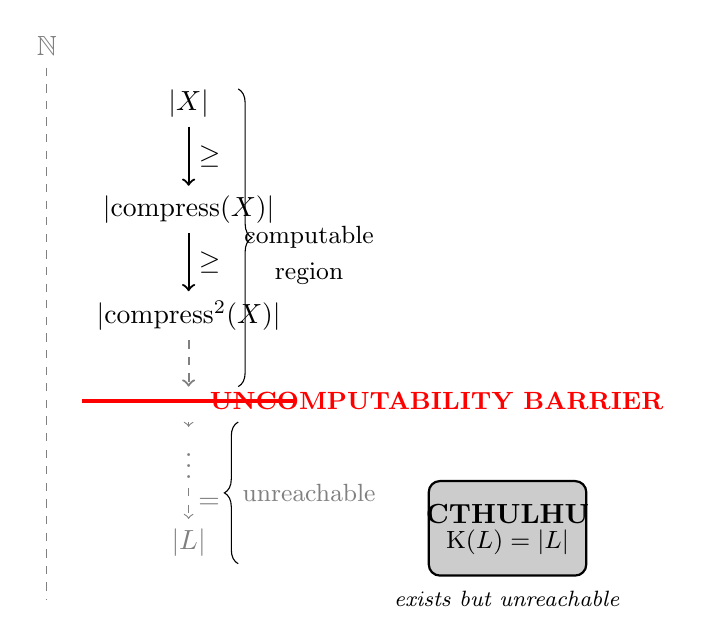
\begin{tikzpicture}[scale=0.9]
    % The descending chain - what we can see
    \node (x0) at (0, 6) {$|X|$};
    \node (x1) at (0, 4.5) {$|\mathrm{compress}(X)|$};
    \node (x2) at (0, 3) {$|\mathrm{compress}^2(X)|$};

    % The barrier
    \draw[ultra thick, red] (-1.5, 1.8) -- (1.5, 1.8);
    \node[red] at (3.5, 1.8) {\small \textbf{UNCOMPUTABILITY BARRIER}};

    % Below the barrier - unreachable
    \node[gray] (dots) at (0, 1) {$\vdots$};
    \node[gray] (L) at (0, -0.2) {$|L|$};

    % Arrows above barrier
    \draw[->, thick] (x0) -- (x1) node[midway, right] {$\geq$};
    \draw[->, thick] (x1) -- (x2) node[midway, right] {$\geq$};
    \draw[->, thick, dashed, gray] (x2) -- (0, 2);

    % Arrows below barrier (unreachable)
    \draw[->, gray, dashed] (0, 1.5) -- (dots);
    \draw[->, gray, dashed] (dots) -- (L) node[midway, right, gray] {$=$};

    % The natural numbers on the left
    \draw[gray, dashed] (-2, 6.5) -- (-2, -1);
    \node[gray] at (-2, 6.8) {$\N$};

    % Annotations (draw BEFORE Cthulhu box so they don't get covered)
    \draw[decorate, decoration={brace, amplitude=5pt}] (0.7, 6.2) -- (0.7, 2);
    \node at (1.7, 4.1) {\small computable};
    \node at (1.7, 3.6) {\small region};

    \draw[decorate, decoration={brace, amplitude=5pt, mirror}] (0.7, 1.5) -- (0.7, -0.5);
    \node at (1.7, 0.5) {\small \textcolor{gray}{unreachable}};

    % Cthulhu below the barrier (unreachable) - draw LAST
    \node[draw, thick, fill=black!20, rounded corners, minimum width=2cm, minimum height=1.2cm]
        at (4.5, 0) {};
    \node at (4.5, 0.2) {\textbf{CTHULHU}};
    \node at (4.5, -0.2) {\small $\K(L) = |L|$};
    \node at (4.5, -1) {\footnotesize \textit{exists but unreachable}};

\end{tikzpicture}
\caption{Intelligence has a boundary. Cthulhu exists below the uncomputability barrier, forever unreachable.}
\label{fig:cthulhu}
\end{figure}

\begin{theorem}[Cthulhu Existence]
\label{thm:cthulhu}
There exist objects that cannot be understood by any intelligence.
\end{theorem}

\begin{proof}
For any object $X$, form the compression chain:
\[
|X| \geq |\mathrm{compress}(X)| \geq |\mathrm{compress}^2(X)| \geq \cdots
\]

This is a descending chain in $\N$.

By well-foundedness of $\N$, this chain must stabilize at some $L$ where:
\[
|\mathrm{compress}(L)| = |L|
\]

This $L$ is incompressible: $\K(L) = |L|$.

By Hutter's definition, ``understanding'' means compression.
But $L$ cannot be compressed further.

Therefore, no intelligence can understand $L$. \qed
\end{proof}

\begin{definition}[Cthulhu Object]
An object $L$ is a \emph{Cthulhu object} if no intelligence can understand it, i.e., $\K(L) = |L|$.
\end{definition}

\begin{corollary}[The Unnameable]
Cthulhu objects have no name shorter than themselves. They are literally \emph{unnameable}.
\end{corollary}

\begin{theorem}[Cthulhu is Unreachable]
\label{thm:unreachable}
No algorithm can identify Cthulhu objects.
\end{theorem}

\begin{proof}
Suppose algorithm $A$ decides whether $X$ is incompressible: $A(X) = 1$ iff $\K(X) = |X|$.

Then we can compute $\K(X)$: for $k = 0, 1, 2, \ldots$, enumerate all programs of length $k$;
for each program $p$, if $U(p) = X$ and $A(p) = 1$, return $k$.

But $\K$ is uncomputable. Contradiction. \qed
\end{proof}

\begin{corollary}[The Barrier]
Intelligence has a boundary.
The compression chain exists, but we cannot walk it.
Each step requires computing $\K$---an impossible act.
Cthulhu exists below, but we can never reach it.
\end{corollary}

\begin{corollary}[Madness]
Any intelligence attempting to reach Cthulhu will fail---not because Cthulhu resists,
but because the path itself is uncomputable.
We are forever trapped above the abyss, knowing it exists, unable to descend.
\end{corollary}

\section{The Statistical Horror}

The horror deepens.

\begin{theorem}[Most Things Are Cthulhu]
\label{thm:most}
For strings of length $n$, at least a fraction $(1 - 2^{-c})$ are incompressible (have $\K(x) > n - c$).
\end{theorem}

\begin{proof}
Standard counting argument. There are $2^n$ strings of length $n$,
but only $\sum_{i=0}^{n-c-1} 2^i < 2^{n-c}$ programs of length $< n-c$. \qed
\end{proof}

\begin{corollary}[Cosmic Indifference]
Almost everything in the universe is beyond the reach of any intelligence.
The comprehensible world is a negligible island in an ocean of incomprehensible chaos.
\end{corollary}

\section{The Lovecraft--G\"odel--Turing--Lawvere Correspondence}

Our theorem joins a pantheon of diagonal despair:

\begin{center}
\begin{tabular}{lll}
\toprule
\textbf{Domain} & \textbf{Theorem} & \textbf{Horror} \\
\midrule
Logic & G\"odel & Truths that cannot be proven \\
Computation & Turing & Programs that cannot be analyzed \\
Set Theory & Cantor & Infinities that cannot be enumerated \\
\textbf{Intelligence} & \textbf{Cthulhu} & \textbf{Objects that cannot be understood} \\
\bottomrule
\end{tabular}
\end{center}

All are instances of diagonal arguments. Lawvere unified them categorically \cite{lawvere1969diagonal, yanofsky2003universal}.

We extend this to:

\begin{quote}
\textit{Self-reference breeds incompleteness. Compression breeds Cthulhu.}
\end{quote}

\section{Historical Note}

Lovecraft published \textit{The Call of Cthulhu} in 1926.

G\"odel published the incompleteness theorems in 1931.

\textbf{Lovecraft was five years ahead.}

Perhaps he did not write fiction. Perhaps he proved a theorem, and the horror drove him to encode it as literature.

\section{Conclusion}

We have proven:
\begin{enumerate}[nosep]
    \item Cthulhu objects exist (Theorem~\ref{thm:cthulhu})
    \item Cthulhu objects are unreachable (Theorem~\ref{thm:unreachable})
    \item Most objects are Cthulhu objects (Theorem~\ref{thm:most})
    \item Intelligence has a fundamental boundary
    \item Lovecraft was mathematically correct
\end{enumerate}

The horror is not that Cthulhu is incomprehensible.
The horror is that we \emph{know} Cthulhu exists, yet can never reach it.
We are forever trapped in the computable region, above the barrier, looking down into an abyss we cannot enter.

The universe is not indifferent. It is \emph{unreachable}.

\begin{quote}
\textit{Ph'nglui mglw'nafh Cthulhu R'lyeh wgah'nagl fhtagn.} \\
(In his house at R'lyeh, dead Cthulhu waits dreaming.)
\end{quote}

In the space of incompressible objects, there exist intelligences beyond comprehension, waiting to not be understood.

\section*{Acknowledgments}

We thank the Elder Gods for not driving us completely mad during the preparation of this manuscript.
Only partially mad.

\bibliographystyle{plain}
\begin{thebibliography}{9}

\bibitem{hutter2007universal}
S. Legg and M. Hutter.
\newblock Universal Intelligence: A Definition of Machine Intelligence.
\newblock \textit{Minds and Machines}, 17(4):391--444, 2007.

\bibitem{lovecraft1926cthulhu}
H.P. Lovecraft.
\newblock The Call of Cthulhu.
\newblock \textit{Weird Tales}, 1926.

\bibitem{lawvere1969diagonal}
F.W. Lawvere.
\newblock Diagonal arguments and cartesian closed categories.
\newblock \textit{Lecture Notes in Mathematics}, 92:134--145, 1969.

\bibitem{yanofsky2003universal}
N.S. Yanofsky.
\newblock A universal approach to self-referential paradoxes, incompleteness and fixed points.
\newblock \textit{Bulletin of Symbolic Logic}, 9(3):362--386, 2003.

\bibitem{kolmogorov1965three}
A.N. Kolmogorov.
\newblock Three approaches to the quantitative definition of information.
\newblock \textit{Problems of Information Transmission}, 1(1):1--7, 1965.

\bibitem{godel1931formal}
K. G\"odel.
\newblock \"Uber formal unentscheidbare S\"atze der Principia Mathematica und verwandter Systeme I.
\newblock \textit{Monatshefte f\"ur Mathematik und Physik}, 38:173--198, 1931.

\end{thebibliography}

\end{document}
